% ch05-soundness-completeness.tex — Soundness and Completeness as Set Relations
% Shows E (entailed) and A (algorithm output) with subset relationships.
% Pedagogical purpose: make A⊆E / E⊆A visually intuitive.
\documentclass[tikz,border=5pt]{standalone}
\usepackage{fontspec}
\setmainfont{Times New Roman}
\usepackage{unicode-math}
\setmathfont{Cambria Math}
\usetikzlibrary{shapes.geometric,shapes.misc,positioning,fit,backgrounds,arrows.meta}

\begin{document}
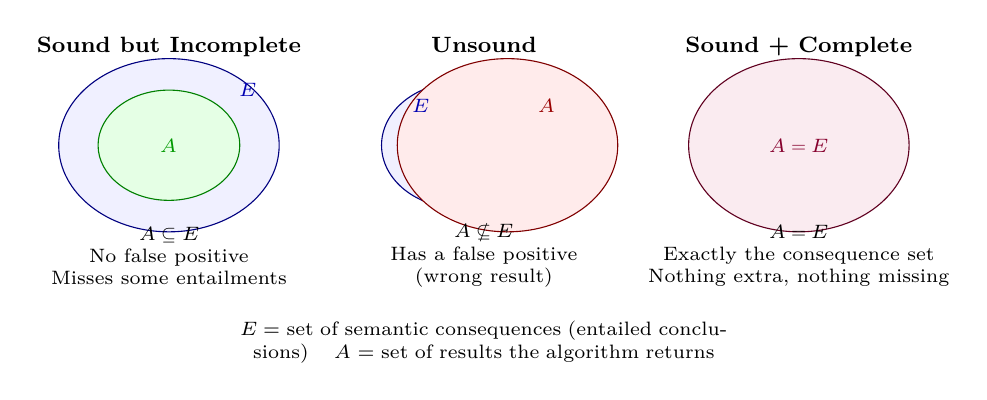
\begin{tikzpicture}[
  setcircle/.style={ellipse,draw,minimum width=2.8cm,minimum height=2.2cm,
                    font=\small,inner sep=2pt},
  label/.style={font=\scriptsize,align=center},
  title/.style={font=\footnotesize\bfseries,anchor=north},
]

% === Case 1: Sound but Incomplete ===
\node[title] at (-4.0,2.8) {Sound but Incomplete};

\node[setcircle,fill=blue!6,draw=blue!50!black] (E1) at (-4.0,1.3) {};
\node[setcircle,fill=green!10,draw=green!50!black,minimum width=1.8cm,minimum height=1.4cm] (A1) at (-4.0,1.3) {};

\node[font=\scriptsize,text=blue!70!black] at (-3.0,2.0) {$E$};
\node[font=\scriptsize,text=green!60!black] at (-4.0,1.3) {$A$};
\node[label] at (-4.0,-0.1) {$A \subseteq E$\\No false positive\\Misses some entailments};

% === Case 2: Unsound ===
\node[title] at (0,2.8) {Unsound};

\node[setcircle,fill=blue!6,draw=blue!50!black,minimum width=2.0cm,minimum height=1.6cm] (E2) at (-0.3,1.3) {};
\node[setcircle,fill=red!8,draw=red!50!black] (A2) at (0.3,1.3) {};

\node[font=\scriptsize,text=blue!70!black] at (-0.8,1.8) {$E$};
\node[font=\scriptsize,text=red!60!black] at (0.8,1.8) {$A$};
\node[label] at (0,-0.1) {$A \not\subseteq E$\\Has a false positive\\(wrong result)};

% === Case 3: Sound + Complete ===
\node[title] at (4.0,2.8) {Sound + Complete};

\node[setcircle,fill=purple!8,draw=purple!50!black] (EC3) at (4.0,1.3) {};
\node[font=\scriptsize,text=purple!70!black] at (4.0,1.3) {$A = E$};

\node[label] at (4.0,-0.1) {$A = E$\\Exactly the consequence set\\Nothing extra, nothing missing};

% Bottom note
\node[font=\scriptsize,align=center,text width=10cm] at (0,-1.2)
  {$E$ = set of semantic consequences (entailed conclusions) \quad
   $A$ = set of results the algorithm returns};

\end{tikzpicture}
\end{document}
